% xetex compatible variant that support TTF fonts according to company rules
\documentclass[ignorenonframetext, professionalfonts, hyperref={unicode}]{beamer}

\usetheme{Epam}

\usepackage{fontspec}
\setsansfont{SourceSansPro-Regular}
%\setbeamerfont{frametitle}{family=\fontspec{Oswald}}
\setbeamerfont{frametitle}{family=\fontspec{Oswald}}
\setbeamerfont{block title}{family=\fontspec{Oswald}}

%\setmainfont{Times New Roman}
\defaultfontfeatures{Mapping=tex-text}
\defaultfontfeatures{Ligatures=TeX}

%\setsansfont{Arial}
%\setromanfont{Trebuchet MS}

\usepackage{cmap}
\usepackage{graphicx}

\usepackage{textcomp}

\usepackage{beamerthemesplit}

\usepackage{ulem}

\usepackage{verbatim}
\usepackage{import}

\usepackage{listings}
\lstloadlanguages{bash}

\lstset{escapechar=`,
	captionpos=b,
	extendedchars=false,
	language=sh,
%	frame=single,
	tabsize=2, 
	columns=fullflexible, 
%	basicstyle=\scriptsize,
	keywordstyle=\color{blue}, 
	commentstyle=\itshape\color{brown},
%	identifierstyle=\ttfamily, 
	stringstyle=\mdseries\color{green}, 
	showstringspaces=false, 
	numbers=left, 
	numberstyle=\footnotesize, 
	breaklines=true, 
	inputencoding=utf8,
	keepspaces=true,
	morekeywords={u\_short, u\_char, u\_long, in\_addr}
	}

\definecolor{darkgreen}{cmyk}{0.7, 0, 1, 0.5}

\lstdefinelanguage{diff}
{
    morekeywords={+, -},
    sensitive=false,
    morecomment=[l]{//},
    morecomment=[s]{/*}{*/},
    morecomment=[l][\color{darkgreen}]{+},
    morecomment=[l][\color{red}]{-},
    morestring=[b]",
}

\author[Epam]{{\bf Epam}\\Low Level Programming Department}

%\institution[EPAM]{EPAM}
%\logo{\includegraphics[width=1cm]{logo.png}}

\graphicspath{{../../slides/cmdline/clipart/}{../../slides/bash/clipart/}}

\bibliographystyle{unsrt}
\setbeamertemplate{bibliography item}{\insertbiblabel}

\AtBeginSection[]{%
  \begin{frame}<beamer>
    \frametitle{}
    \tableofcontents[
        sectionstyle=show/shaded, hideallsubsections ]
  \end{frame}
  \addtocounter{framenumber}{-1}% If you don't want them to affect the slide number
}

% \regex for regular expressions
\newcommand{\regex}[1]{ %
\expandafter{$\ulcorner{\color{blue}\texttt{#1}}\lrcorner$} %
}


%\title[bash]{Bourne again shell}
\title{Введение в GNU/Linux}

%%%%%%%%%%%%%%%%%%%%%%%%%%%%%%%%%%%%%%%%%%%%%%%%%
%%%%%%%%%% Begin Document  %%%%%%%%%%%%%%%%%%%%%%
%%%%%%%%%%%%%%%%%%%%%%%%%%%%%%%%%%%%%%%%%%%%%%%%%

\begin{document}

\begin{frame}
	\frametitle{BASH}
	\titlepage
	\vspace{-0.5cm}
	\begin{center}
	%\frontpagelogo
	\end{center}
\end{frame}

\begin{frame}
	\tableofcontents
%	[hideallsubsections]
\end{frame}

%%%%%%%%%%%%%%%%%%%%%%%%%%%%%%%%%%%%%%%%%   
%%%%%%%%%% Content starts here %%%%%%%%%%
%%%%%%%%%%%%%%%%%%%%%%%%%%%%%%%%%%%%%%%%%


\section{Write and run shell script}
\mode<all>{\begin{frame}{Преимущества автоматизации для сложных задач}
    \begin{center}
      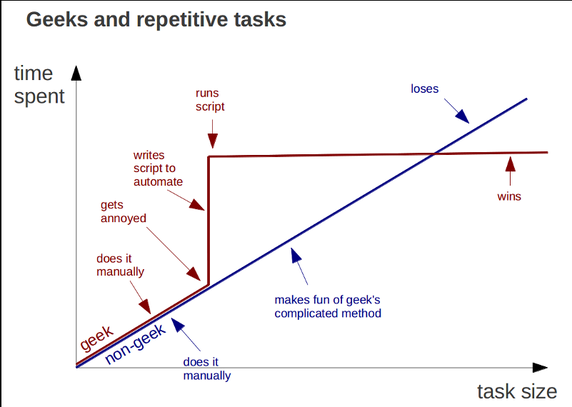
\includegraphics[width=3.6in]{view_automate_geek_vs_nongeek}
    \end{center}
\end{frame}

}
\mode<all>{\begin{frame}[fragile]
\frametitle{ Цикл until. Пример.}
  \begin{block}{Ожидаем хост после перезагрузки.}
    \begin{lstlisting}[language=sh,frame=single]
until ping -q -c 3  $host 1>/dev/null 2>&1 && nc -z $host 22
do 
   sleep 1
   echo unavailable;
done
\end{lstlisting}
  \end{block}
\end{frame}
}
\mode<all>{\begin{frame}
  \frametitle{Bash против скриптовых языков}
  \begin{itemize}
   \item В bash трудно делать сложные структуры данных
   \item В bash нет типизации переменных
   \item Но! В bash очень просто организовывать взаимодействие внешних программ
   \item Stream programming \texttt{(a | b | c )}
  \end{itemize}
\end{frame}

\begin{frame}
  \frametitle{Когда использовать bash}
  \begin{columns}
   \column{0.5\textwidth}
    \begin{center}
     {\Large Использовать}
    \end{center}
    \begin{itemize}
      \item Прототипирование
      \item Системные скрипты, обертки
      \item Автоматизация консоли
    \end{itemize}
   \column{0.5\textwidth}
    \begin{center}
     {\Large Не использовать}
    \end{center}
    \begin{itemize}
      \item Критичные по скорости (интерпретатор)
      \item GUI
      \item Сложные структуры данных (двумерный массив, бинарные деревья, нет типизации переменных)
    \end{itemize}
  \end{columns}
\end{frame}
}
\mode<all>{\begin{frame}[fragile]{Оболочка операционной системы}

     \begin{block}{Оболочка операционной системы}
     (от англ. shell «оболочка») \alert{интерпретатор команд} операционной системы, обеспечивающий интерфейс для взаимодействия пользователя с функциями системы.  
     \end{block}

     Что такое Unix shell?
     \begin{itemize}
        \item Обычная программа, запускающаяся после входа в систему
	\pause
        \item Интерактивный командный интерпретатор
	\pause
        \item Платформа интеграции для утилит (glue-language)
	\pause
        \item Язык программирования
	\pause
        \item Макропроцессор (программа выполяняющая преобразование текста)
     \end{itemize}

        Например:
	\pause
	Оболочки из Windows --  cmd.exe, PowerShell

	Минимальный дистрибутив Linux -- ядро + shell 

\end{frame}
}
\mode<all>{\begin{frame}[fragile]{Задание. Виды оболочек.}
Получить список установленных оболочек.
\begin{lstlisting}[language=bash]
cat /etc/shells
ls -l <filename> # для каждого элемента /etc/shells
readlink -e <filename> 
\end{lstlisting}
Запустить любую из установленных оболочек. 

\begin{lstlisting}[language=bash]
/usr/bin/ksh 
/usr/bin/zsh 
/usr/bin/fish
\end{lstlisting}

\alert{Bash} - (Bourne-again shell) оболочка по умолчанию в большинстве дистрибутивов Linux.

выход из оболoчки  Ctrl-D, либо exit
\end{frame}
}
\mode<all>{\begin{frame}[fragile]
  \frametitle{Скрипты}
 
  \begin{block}<1->{Shell Script, определение}  

    Последовательность команд Shell.

    Разделитель: перевод строки, \textquotedbl ; \textquotedbl
  \end{block}

  \begin{block}<2->{shebang}
    \verb+#!something+ или чем мы запускаем скрипт. 
    
    По умолчанию : \verb+#!/bin/sh+
  
    Всегда первая строка скрипта.

    Фактически: \verb+/bin/sh scriptname+
  \end{block}

  \begin{block}<3->{Парадоксальные примеры}
    \verb+#!/bin/rm+

    \verb+#!/bin/awk -f+

    \verb+#!/bin/less+
  \end{block}

\end{frame}
}
\mode<all>{\begin{frame}[fragile]
  \frametitle{Запуск скриптов}
  \begin{enumerate} 
    \item \verb+sh scriptname+
    \item \verb-chmod +x script- \newline \verb+./script+
    \item из каталогов в переменной PATH 
      \newline \verb+echo $PATH+
      \newline \verb+~/bin+ (если есть)
      \newline \verb+/usr/local/bin+
    \item в текущей копии shell\footnote{ Остальные способы - запускают новый shell}
      \newline \verb+. ./script+
      \newline \verb+source script+\footnote{ Несовместимо с POSIX. Происходит из ksh. Добавляет текущий каталог к списку путей}
  \end{enumerate}
\end{frame}
}

%\section{Manipulate the different I/O streams  with I/O Redirection}
%\mode<all>{\begin{frame}[fragile]
	\frametitle{stdin, stdout, stderr}
     C каждым процессом связаны потоки ввода-вывода - файловые дeскрипторы stdin, stdout, stderr.
    \begin{block}{Пример. Номера файловых дeскрипторов и устройств. }
                    \begin{lstlisting}
echo /dev/std*
echo /dev/std* | xargs -t -n 1 readlink
lsof -ap $BASHPID -d 0,1,2
                    \end{lstlisting}
    \end{block}
\end{frame}
}
%\mode<all>{

\begin{frame}{Конвееры}
%  \textbf{Цель} -- максимальная модульность: большое количество простых приложений, взаимодействующих друг с другом для решения задач
  \only<1>{
  \begin{center}
    \includegraphics[width=1.2in]{../../slides/cmdline/process}
  \end{center}
  }
  \only<2>{
    \begin{center}
      \includegraphics[width=3.6in]{../../slides/cmdline/processes}
    \end{center}
  }
  \begin{itemize}
    \item <1-> Каждое приложение открывает 3 стандартных файловых дескриптора (file descriptor) \alert{stdin (fd 0)}, \alert{stdout(fd 1)}, \alert{stderr (fd 2) }
    \item <2-> Приложения могут работать как фильтр из \alert{STDIN} в \alert{STDOUT}, можно объединять несколько приложений в конвейер
    \item <2-> Синтаксис {\tt <app1> | <app2>}
  \end{itemize}
\end{frame}
}
%\mode<all>{\begin{frame}{Перенаправления в файл}

\begin{itemize}
  \item Перенаправление stdout FD=1
    \begin{itemize}
      \item С созданием нового файла

        {\tt command > file}\\
		Например {\tt cat file1 file2 > file3}
      \item С дополнением существующего

		  {\tt command >\phantom{}>  file}
    \end{itemize}
    \pause
  \item Перенаправления stdin FD=0

    {\tt command < file}
    \pause
  \item Перенаправления stderr FD=2

    {\tt command1 2>\&1 | command2}

   {\tt command 1>file 2>\&1}

   {\tt command 2>file 1>\&2}
\end{itemize}

\end{frame}
}
%\mode<all>{\begin{frame}{Применение перенаправления потоков.}
Работает с любым типом файлов.
\begin{itemize}
  \item Создать новый файл или обнулить сущствующий >
  \item Перенаправить длинный вывод команды в файл >
  \item Молчаливое выполнение команды >/dev/null 
  \item Чтение из спецфайла </dev/urandom, /dev/zero 
  \item Чтение из данных из файла <
  \item Настройка системы. echo >  определенные файлы в /proc/ или /sys/
  \item cat /dev/zero > /dev/sda - удалить систему
\end{itemize}

\end{frame}
}
%\mode<all>{\begin{frame}[fragile]
	\frametitle{Перенаправление ввода/вывода}

	\begin{itemize}
		\item ``>'' -- Перенаправление в файл
			\begin{block}{Пример}
				\begin{lstlisting}
echo stdout > test.txt
				\end{lstlisting}
			\end{block}
		\item ``>\&'' -- Перенаправление в другой дескриптор
			\begin{block}{Пример}
				\begin{lstlisting}
(echo stdout; echo stderr >&2) > test.txt
				\end{lstlisting}
			\end{block}
	\end{itemize}

\end{frame}
}
%\mode<all>{\begin{frame}[fragile]
	\frametitle{Перенаправление ввода/вывода}

	\begin{itemize}

		\item ``\&>''
			\begin{block}{Пример}
				\begin{lstlisting}
(echo stdout; echo stderr >&2) &> test.txt
\end{lstlisting}
			\end{block}
		
		\item ``>{}>'' -- Добавление в файл
			\begin{block}{Пример}
				\begin{lstlisting}
echo stdout >> test.txt
\end{lstlisting}
			\end{block}

		\item ``<'' -- Чтение из файла
			\begin{block}{Пример}
				\begin{lstlisting}
cat < test.txt
\end{lstlisting}
			\end{block}
	\end{itemize}

\end{frame}
}
%\mode<all>{\begin{frame}[fragile]
	\frametitle{Перенаправление ввода/вывода}

	\begin{itemize}

		\item ``<<'' -- Here-документ

		\item ``<>'' -- Открывает файловый дескриптор из файла/другого дескритора
			\begin{block}{Пример}
				\begin{lstlisting}
exec 3<>test.txt; echo test >&3;  cat <test.txt
				\end{lstlisting}
			\end{block}
			
		\item ``n<\&-'' -- Закрывает файловый дескриптор
			\begin{block}{Пример}
				\begin{lstlisting}
exec 3<&-; echo test >&3
				\end{lstlisting}
			\end{block}
			
		\item ``|'' -- pipe
	\end{itemize}

\end{frame}
}

%\mode<all>{\begin{frame}[fragile]
	\frametitle{Начало скрипта \#!}

        Конструкция позволяет использовать скрипты, как системные команды. 
        Первая cтрока игнорируется интерпретатором, т.к. \# - комментарий

	\begin{block}{Sha-Bang, shebang, hasbang}
		\begin{lstlisting}
#!/bin/bash
		\end{lstlisting}
	\end{block}

	\begin{block}{Режим совместимости с POSIX}
		\begin{lstlisting}
#!/bin/sh
		\end{lstlisting}

	\end{block}

\end{frame}
}

\section{Understand expansion}
% bash macroprocessor
\mode<all>{\begin{frame}{Встроенный макропроцессор}

\begin{itemize}
    \item brace expansion  \alert{\{ \}} фигурные скобки
    \item tilde expansion \alert{\textasciitilde{}file}
    \item parameter and variable expansion \alert{\$name}, \alert{\$\{name\}} 
    \item command substitution \alert{\$( )} круглые скобки
    \item arithmetic expansion \alert{(())}, \alert{\$(())} двойные круглые скобки
    \item word splitting \alert{"}, \alert{'}, \alert{\textvisiblespace} пробел
    \item filename expansion (globbing) \alert{*}, \alert{?}, \alert{[]} 
\end{itemize}
    
\end{frame}
}
% brace expansion
\mode<all>{\begin{frame}
	\frametitle{Спецсимвол фигурная скобка}

	\begin{block}{Фигурные скобки и склеивание с помощью ``,``}
		\begin{itemize}
			\item Посмотреть на результат выполнения команды \\
				{\tt echo \{A,B,C\}:\{1,2,3\}}
				\pause
			\item Посмотреть на результат выполнения команды \\
				{\tt ls -l \{,/usr\}/\{bin,sbin\}/*sh}
		\end{itemize}
	\end{block}

	\pause

	\begin{block}{Фигурные скобки и перечисления с помощью ``..``}
		\begin{itemize}
			\item Посмотреть на результат выполнения команды \\
				{\tt echo \{a..d\}:\{-10..10\}}
		\end{itemize}
	\end{block}

\end{frame}

\begin{frame}{Спецсимвол фигурная скобка}

Применяют как простой генератор строк и последовательностей
\begin{itemize}
    \item в циклах 
    \item для создания вложенных директорий 
    \item генерации файлов по шаблону. Файл не обязательно существует на в файловой системе.
\end{itemize}
    
\end{frame}
}
% parameters expansion
\mode<all>{\begin{frame}
	\frametitle{Специальные параметры}

	Позиционные параметры - передаются при запуске скрипта, средство передачи данных в скрипт.

        Например: 

        ./myscript.sh file.txt /tmp/

        \$1 file.txt

        \$2 /tmp/
        
	\begin{itemize}
		\item \$0-9, \$\{10\}.. -- значение соответствующего параметра
		\item \$\# -- количество переданных параметров
		\item \$* -- представляется, как одна строка
		\item \$@ -- каждый параметр, как отдельная строка
	\end{itemize}

\end{frame}


\begin{frame}[fragile]
	\frametitle{shift}

	Встроенная команда сдвига параметров влево.

        По умолчанию сдвигает на один параметр.

	В качестве параметра может принимать число -- на сколько параметров сдвигать.

\begin{lstlisting}
shift [num]
\end{lstlisting}

\end{frame}


% \begin{frame}
%	\frametitle{Задание}
%
%	\begin{enumerate}
%		\item Написать скрипт,  который выдает количество переданных параметров
%			\pause
%		\item Вывести на экран имя команды
%			\pause
%		\item Сделать symlink на скрипт и запустить
%			\pause
%		\item Вывести на экран первых 3 параметра
%			\pause
%		\item Передать строку "I am user \$USER" в качестве параметра
%			\begin{itemize}
%				\item Без экранирования
%				\item С экранированием ''
%				\item С экранированием '
%			\end{itemize}
%			\pause
%		\item Добавить shift перед выводом параметров
%	\end{enumerate}
%\end{frame}
%

}
% globbing
% \mode<all>{\begin{frame}[fragile]
  \frametitle{Подстановочные символы путей (globbing)}

  \alert{Wildcard characters} - спецсимволы в параметрах команд, раскрываемые в путь и имя файла самим интерпретатором перед тем, как запустить команду на выполнение. \pause


  \begin{itemize}
    \item \alert{*} - любое количество любых символов
\begin{lstlisting}[basicstyle=\normalsize]
        echo *
        ls /u*
\end{lstlisting} \pause
    \item \alert{[]} - символ из перечисления\footnote{об интервалах - в разделе о регулярных выражениях}
\begin{lstlisting}[basicstyle=\normalsize]
        echo .[bp]*
        ls /sys/*/net/
\end{lstlisting} \pause
    \item \alert{?} - любой одиночный символ
\begin{lstlisting}[basicstyle=\normalsize]
        ~$ echo ?i*
\end{lstlisting} 
  \end{itemize}

\end{frame}

}

% symbols escape
% asterics example
% \mode<all>{\begin{frame}[fragile]
	\frametitle{Задание. Строка спецсимволов}
Вывести символ * 10 раз.
				\begin{lstlisting}
echo *********
                                \end{lstlisting}
\end{frame}
}

%\mode<all>{\begin{frame}[fragile]
	\frametitle{Экранирование}

	\begin{columns}
		\column{0.5\textwidth}
		\begin{itemize}
			\item Экранирование одного символа \alert{ \textbackslash }
			\item Частичное экранирование \alert{ '' }
			\item Полное экранирование \alert{ ' }
		\end{itemize}
		\pause
		\column{0.5\textwidth}
		Спецзначения для echo и sed
		\begin{itemize}
			\item \textbackslash{n} -- новая строка
			\item \textbackslash{r} -- возврат каретки
			\item \textbackslash{t} -- табуляция
			\item \textbackslash{v} -- вертикальная табуляция \\
				\small\begin{lstlisting}
echo -e "test \v test \v test"
				\end{lstlisting}
			\item \textbackslash{b} -- перемещение на 1 символ назад
			\item \textbackslash{a} -- звуковой сигнал
			\item \textbackslash{0xxx} -- 8-миричное число
			\item \textbackslash{xXX} -- 16-ричное число
		\end{itemize}
	\end{columns}

\end{frame}
}
% spaces
\mode<all>{\begin{frame}[fragile]
	\frametitle{Задание. Обработка пробелов.}
Сравнить результаты команд для имени, которое содержит пробелы
				\begin{lstlisting}
ls a long file name with spaces
ls "a long file name with spaces" 
				\end{lstlisting}
\end{frame}
}

%exec
%\mode<all>{\begin{frame}
	\frametitle{exec}

	Заменяет текущий shell переданной командой. 

	Часто используется для переназначения файловых дескрипторов.

\end{frame}
}

\section{Use variables in scripts}
\mode<all>{%% Vars


\begin{frame}
	\frametitle{Переменные}
	\large\center{Нетипизированные!!!}

	Для прямого обращения необходимо использовать префикс \\
	\center{\Large{\tt \$}}

	Фигурные скобки используют для отделения от текста:\\
	\center{\tt \$VARrest != \$\{VAR\}rest}

	%\bigskip
	
	\begin{alertblock}{Используют без префикса}
		\begin{itemize}
			\item в объявлении declare var
			\item в присвоении declare var=10
			\item чтение в командe read var
			\item удаление unset var
			\item в арифметических операциях {\tt (( a=b+c ))}
		\end{itemize}
	\end{alertblock}
\end{frame}

\begin{frame}[fragile]
	\frametitle{Задание. Присвоить переменной значение.}

	\begin{lstlisting}
#!/bin/bash

VAR=string
echo $VAR
	\end{lstlisting}


	\begin{block}{Изменить и посмотреть на результат.}
		\begin{itemize}
			\item Добавить пробел до знака ''{\tt =}''
			\item Добавить пробел после знака ''{\tt =}''
			\item Присвоить переменной VAR значение: I love \$\$\$!
			\item Создать переменные с другим именем и значением var 1var \_var var1
		\end{itemize}
	\end{block}

\end{frame}

\begin{frame}[fragile]
	\frametitle{Косвенное обращение к переменной}

	Косвенное (indirect) обращение к переменной: {\tt \$\{!VARIABLE\}}

	\begin{block}{Пример}
		\begin{lstlisting}
#!/bin/bash 
num=$# 
lastarg=${!num} 
echo $num $lastarg
		\end{lstlisting}
	\end{block}

\end{frame}


\begin{frame}
	\frametitle{Типы переменных}
	\begin{itemize}
		\item Локальные\\
		    Область видимости -- текущая программа, функция или субшелл
		\item Окружения
		\item Позиционные параметры
	\end{itemize}
\end{frame}



\begin{frame}
	\frametitle{Внешние переменные}

	\center{Наследование внешней переменной}

	\begin{itemize}
		\item export
		\item Переданное в командной строке \\
			\begin{block}{Пример}
				{\tt TEST=123 make}
			\end{block}
	\end{itemize}
\end{frame}


\begin{frame}[fragile]
	\frametitle{Специальные переменные}

	Часто используемые в скриптах:

	\begin{itemize}
		\item Разделитель \$IFS
		\item Директории -- домашняя \$HOME и текущая \$PWD
		\item UID пользователя -- \$UID
		\item ID процесса -- \$\$
		\item Имя хоста -- \$HOSTNAME
		\item Вид командной строки: \$PS1 -- \$PS4
		\item Локализация
			\begin{itemize}
				\item Используемый язык \$LANG
				\item Локализация \$LC\_ALL
					\begin{block}{Пример}
						\begin{lstlisting}
ls -l 
LC_ALL=C ls -l
						\end{lstlisting}
					\end{block}
			\end{itemize}
	\end{itemize}

\end{frame}



}

%exit code
\mode<all>{\begin{frame}[fragile]

  \Large{\alert{Код возврата (RETURN CODE)}}: \newline 
  \normalsize{результат выполнения у любой команды Shell}
  \newline

  Shell return code:
  \begin{itemize}
    \item 0 - выполнено успешно
    \item не 0 - ошибка
    \item Код возврата доступен через переменную \$?
  \end{itemize}

	\pause
	\begin{block}{Пример}
		\begin{lstlisting}
/bin/true; echo $?
/bin/false; echo $?
		\end{lstlisting}
	\end{block}

	Скрипт возвращает код последней команды, поэтому для корректного выхода необходимо использовать команду {\tt exit 0} - в случае успеха

\end{frame}
}
%\mode<all>{\begin{frame}[fragile]
  \frametitle{Условное выполнение команд}

  \Large{\alert{Код возврата (RETURN CODE)}}: \newline 
  \normalsize{результат выполнения у любой команды Shell}
  \newline

  Shell return code:
  \begin{itemize}
    \item 0 - выполнено успешно
    \item не 0 - ошибка
  \end{itemize}
  \pause

  Операции над кодом возврата:
  \begin{itemize}
    \item \textquotedbl \verb+&&+ \textquotedbl - логическое И
    \item \textquotedbl \verb+||+ \textquotedbl - логическое ИЛИ
  \end{itemize}
  \pause

  Примеры:
  \begin{itemize}
    \item \verb+ cat /proc/1/environ || echo fail +
    \item \verb+ find /usr/share/doc -name \textquotedbl *.txt \textquotedbl && echo ok+
  \end{itemize}

\end{frame}
}

\section{Tests and conditions}
%\mode<all>{\begin{frame}[fragile]
    \frametitle{ Задание. Выполнить команды.}
\begin{block}{AND}
	\small\begin{lstlisting}
false && echo Not running
true && echo Running
	\end{lstlisting}
\end{block}

\begin{block}{OR}
	\small\begin{lstlisting}
false || echo Running
true || echo Not running
	\end{lstlisting}
\end{block}
\end{frame}
}
%\mode<all>{\begin{frame}[fragile]
    \frametitle{Общий синтаксис}

	\begin{block}{Конструкции для сравнения}
		\begin{itemize}
			\item {\tt \&\&} -- выполнится в случае успеха
			\item {\tt ||} -- выполнится в случае неудачи
		\end{itemize}
	\end{block}

	\begin{verbatim}
команда1 && команда2  или  условие1 && команда2 
команда1 || команда2  или  условие1 || команда2 
команда1 && команда2 && команда3 && ... && командаN
	\end{verbatim}

\end{frame}
}

\mode<all>{\begin{frame}[fragile]{Условный оператор.}

Во время выполнения программы условный оператор позволяет выполнять разные наборы команд в зависимость от условного выражения.
\begin{columns}
  \column{0.6\textwidth}

В bash условное выражение - любая \alert{команда}. \\

Код возврата доступен через переменную \alert{\$?} \\

Поддерживает синтаксические конструкции: \alert{\&\&}, \alert{||}, \alert{if then (else)}, \alert{case}, \alert{select}.
А также cемейство команд для сравнения \alert{test}.

\column{0.4\textwidth}
\center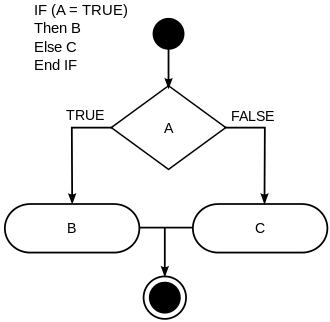
\includegraphics[width=4cm]{If-Then-Else-diagram}

 \end{columns}
    
\end{frame}
}
% Команды сравнения.
\mode<all>{\begin{frame}[fragile]
   \frametitle{Команды сравнения.}

\underline{Выполнить команды:}
	\small\begin{lstlisting}
type -a test [ [[
test -f /etc/ ; echo $? # существует ли файл?
test -d /etc/ ; echo $? # существует ли директория?
	\end{lstlisting}

\pause
\alert{Команда test} сравнивают аргументы в условии. Если условие выполенено успешно, команда возвращет exit code \alert{0} иначе \alert{1}.

Синтаксис:
\begin{verbatim}
test expression 
[expression] 
[[ expression ]]
\end{verbatim}
expression - условное выражение. Синтаксис условного выражения может различаться от типа команды.
Есть несколько типов команд:

\begin{itemize}
    \item встроенные в оболочку test, [
    \item внешние /usr/bin/test, /usr/bin/[
    \item ключевое слово [[
\end{itemize}


\end{frame}
}

\mode<all>{\begin{frame}[fragile]
\frametitle{Что можно сравнивать в условии}

\underline{Выполнить команды:}
	\small\begin{lstlisting}
help test ; help [ ; help [[ # показывает опции для встроенных команды из оболочки
man test  # для внешней команды
\end{lstlisting}
    \pause
	\begin{itemize}
	    \item \alert{!} -- отрицание
	    \item \alert{-z} СТРОКА
	    \item СТРОКА1 \alert{==} СТРОКА2 или СТРОКА1 \alert{=} СТРОКА2
	    \item СТРОКА1 \alert{!=} СТРОКА2
	    \item ЦЕЛОЕ1 \alert{-eq} ЦЕЛОЕ2
	    \item ЦЕЛОЕ1 \alert{-ge} ЦЕЛОЕ2
	    \item ЦЕЛОЕ1 \alert{-lt} ЦЕЛОЕ2
	    \item \alert{-d} ФАЙЛ
	    \item \alert{-e} ФАЙЛ
	    \item \alert{-f} ФАЙЛ
	\end{itemize}

\end{frame}
}
%\mode<all>{\begin{frame}
    \frametitle{Условное выражение}
		\begin{itemize}
			\item Exit status любой программы
			\item Команда test или $[$ ... $]$
			\item $[[$ ... $]]$
			\item Двойные скобки {\bf (( ... ))} и конструкция {\bf let}
		\end{itemize}
\end{frame}
}


%% test and [[ comparison
% \mode<all>{\begin{frame}[fragile]
    \frametitle{ Особенности использования [[ }
    \begin{block}{Кавычки обрабатываются по разному}
	\small\begin{lstlisting}
a="a b c" b="a b c"
[ $a = $b ] && echo $? # ошибка bash: [: too many arguments
[[ $a = $b ]] && echo $? # не нужно брать в кавычки ""
	\end{lstlisting}
    \end{block}

    \begin{block}{ Операторы \&\& AND || OR }
	\small\begin{lstlisting}
[[ "abc" = 1 -a "b" = 2 ]] # syntax error in conditional expression
[[ "abc" = 1 && "b" = 2 ]] # вместо -a использовать &&, -o ||
	\end{lstlisting}
    \end{block}
\end{frame}
}
% \mode<all>{\begin{frame}[fragile]
    \frametitle{ Сравнение по шаблону}
    \begin{block}{ Pattern matching}
	\small\begin{lstlisting}
a="a b c"
[[ $a = a* ]] ; echo $? # строка совпадает с паттерном
[[ $a = d* ]] ; echo $? # символа d нет в строке
[[ $a = "a*" ]] ; echo $? # кaвычки отменяют паттерн
[[ $a =~ "a*" ]] ; echo $? # регулярные выражения
\end{lstlisting}
    \end{block}
\end{frame}
}
% \mode<all>{\begin{frame}[fragile]
	\frametitle{Двойные квадратные скобки [[}

\begin{itemize}
        \item работает только в оболочках bash, zsh, ksh. Команды [ и test доступны в оболочках POSIX.
        \item Ведет себя не как команда, а как ключевое слово
        \item Доступны дополнительные сравнения (на соответствие регулярному выражению) или шаблону
        \item Нет необходимости закавычивать переменные и экранировать скобки \(\)
        \item Внутри можно использовать логические связки \({\tt \&\&, \|, \langle, \rangle}\)
\end{itemize}

\end{frame}
}

\mode<all>{\begin{frame}[fragile]
\frametitle{Синтаксис {\bf if}}

	\begin{columns}
		\column{0.5\textwidth}
	
	\begin{lstlisting}[language=bash]
if command1
then
    OTHER COMMANDS
elif command2
then
    OTHER COMMANDS
else
    OTHER COMMANDS
fi
\end{lstlisting}
		\column{0.5\textwidth}
Варианты форматирования
then отдельной строкой
	\begin{lstlisting}[language=bash]
if command
then OTHER COMMANDS 
fi
\end{lstlisting}

then и if на одной строке
	\begin{lstlisting}[language=bash]
if command; then 
    OTHER COMMANDS
fi
\end{lstlisting}
	\end{columns}

В зависимости от результата выполнения (exit code) command1 выполняется блок команд после then.   

Ключевое слово fi - обязательно

%	\pause
%	{\bf Практическое задание:} \\
%	\begin{itemize}
%
%		\item с помощью конструкции {\bf if} проверить существует ли файловый объект передаваемый в качестве параметра скрипту ({\tt man test})
%		\item если нет, то создать директорию с таким именем
%		\item если cуществует и файл является shell-скриптом ({\tt man file}), то запустить его
%		\item если существует и является директорией, то вывести на экран Top5 по размеру файлов из этой директории, 
%		    отсортированных в порядке убывания ({\tt man ls, man head})
%%	\end{itemize}
%	\end{columns}
\end{frame}
}


%\mode<all>{\begin{frame}[fragile]
\frametitle{case + getopt}
	Внешняя команда для обработки аргументов командной строки.
	\small
	\begin{lstlisting}
SHORTOPTS="af:h"
LONGOPTS="flagA,file:,help"
OPTS=$(getopt -o "$SHORTOPTS" -l "$LONGOPTS" -- "$@")

eval set -- "$OPTS" #  устанавливает $1 $2 ...

while [ $# -gt 0 ] ; do
  case $1 in
    -a|--flagA) FLAGA=$1 ; shift ;;
    -f|--file) FILE=$1; FILENAME="$2"; shift 2 ;;
    -h|--help) echo "Usage:$0 [-a|--flagA] [-h|--help] [-f|--file <filename>]"; exit 0;;
    --) shift; break ;; # skip this one
    *) ;;
  esac
done
\end{lstlisting}
\end{frame}
}
%\mode<all>{\begin{frame}[fragile]
	\frametitle{case + getopts}
	
	Встроенная в bash обработка командной строки.

\begin{lstlisting}[language=sh,frame=single]
while getopts "af:h" Option
do
  case $Option in 
    a) FLAGA=1 ;;
    f) FILE=1
       FILENAME=$OPTARG
       ;;
    h) echo "Usage: $0 [-ah] -f <filename>";;
  esac  
done
shift $((OPTIND-1))
\end{lstlisting}
\end{frame}
}

%\mode<all>{\begin{frame}
\frametitle{Домашнее задание}

	Написать скрипт, который будет создавать файл, 
	записывать туда текущее время и переданную строку,
	используя при этом следующие аргументы командной строки: 

	\begin{enumerate}
		\item -f или -{}-file <имя файла>\\
			если отсутствует имя файла, то выйти с соответствующим сообщением;
		\item -l или -{}-log <строка>\\
			если отсутствует <строка>, то выйти с соответствующим сообщением;
		\item -a или -{}-append \\
			необязательный флаг, указывающий будет ли файл переписан, либо дописан.
	\end{enumerate}

	Cкрипт должен обрабатывать переданные аргументы с использованием {\tt getopt} либо {\tt getopts}.

\end{frame}
}
% select example
%\mode<all>{\begin{frame}[fragile]
\frametitle{Условные операторы: select}

	\small
	\begin{columns}
		\column{0.3\textwidth}

		\begin{lstlisting}[language=sh,frame=single]
select variable [in list]
do
  command...
  break
done 
\end{lstlisting}
		\pause
		\column{0.7\textwidth}
		{\normalsize Пример:}

         \lstinputlisting[language=bash]{../../slides/bash/samples/select.sh}
		\pause
		\center{Удалить в select все [in *] и посмотреть на результат работы.}

	\end{columns}
\end{frame}
2

\section{Repeat operations with loops.}
\mode<all>{\begin{frame}
\frametitle{Основные конструкции для циклов}
  \begin{itemize}
   \item for - цикл просмотра (foreach), цикл со счетчиком 
   \item while, until - цикл с предусловием  
   \item break, continue  - досрочный выход, пропуск итерации
  \end{itemize}
\end{frame}
}

%\mode<all>{\begin{frame}[fragile]
  \frametitle{Циклы for}
  \begin{enumerate}
    \item Стандартная форма
\begin{lstlisting}[language=sh,frame=single]
  for x in list 
  do
    op1
    op2
  done
\end{lstlisting}
    \item Арифметическая форма
\begin{lstlisting}[language=sh,frame=single]
  for (( expr1 ; expr2 ; expr3 )) 
  do 
    op1
    op2
  done
\end{lstlisting}
  \end{enumerate}
\end{frame}
}

\mode<all>{\begin{frame}[fragile]
\frametitle{ Циклы for. Примеры.}
  \begin{block}{Действие над файлами.}
\begin{lstlisting}[language=sh,frame=single]
for file in *
 do md5sum $file
done
\end{lstlisting}
  \end{block}

\begin{block}{Перечисление элементов.}
\begin{lstlisting}[language=sh,frame=single]
for planet in Mars Earth Mercury Saturn
 do echo $planet 
done
\end{lstlisting}
  \end{block}
\end{frame}
}
\mode<all>{\begin{frame}[fragile]
\frametitle{Циклы for. Цифровая последовательность.}
  \begin{block}{Примеры генерации.}
\begin{lstlisting}[language=bash,frame=single]
for num in 1 2 3 4 5 6 7 8 9 10 # простое перечисление 
 do ping 192.168.10.$num
done

for num in $(seq 1 10)  # генерация из внешней команды
 do ping 192.168.10.$num
done

for num in {1..10}  # генерация встроенными средствами
 do ping 192.168.10.$num
done

\end{lstlisting}
  \end{block}
\end{frame}
}
\mode<all>{\begin{frame}[fragile]
\frametitle{Циклы for. Цифровая последовательность.}
  \begin{block}{Арифметический формат (C-like) }
\begin{lstlisting}[language=bash,frame=single]
for ((i=1;i<11;i++))
do 
  echo $i
done  
\end{lstlisting}
  \end{block}

  \begin{block}{Несколько переменных}
    \begin{lstlisting}[language=sh,frame=single]
for ((a=1, b=1; a <= LIMIT ; a++, b++))
do
  echo -n "$a-$b"
done
\end{lstlisting}
  \end{block}
\end{frame}
}
\mode<all>{\begin{frame}[fragile]
\frametitle{ Циклы for. Примеры.}
  \begin{block}{Пустые выражения. Результат по умолчанию 1. }
    \begin{lstlisting}[language=sh,frame=single]
for (( i=1; ; i++))
do
  echo $i 
  [ "$i" -eq 10 ] && break 
done
    \end{lstlisting}
  \end{block}
\end{frame}
}
%\mode<all>{\begin{frame}[fragile]
\frametitle{ Цикл for. Примеры.}
  \begin{block}{Aргументы командной строки.}
    \begin{lstlisting}[language=bash,frame=single]
for arg
 do echo $arg 
done
    \end{lstlisting}
  \end{block}
  \begin{block}{Из переменной. Запись одной строкой.}
    \begin{lstlisting}[language=bash,frame=single]
for name in "$users" ; do echo $name ; done
    \end{lstlisting}
  \end{block}
\end{frame}
}
% while
\mode<all>{\begin{frame}[fragile]
\frametitle{Циклы while,until}
\begin{lstlisting}[language=sh,frame=single]
while expr1; ... exprN
do
 op
done
\end{lstlisting}
Применяются когда нужно повторять до выполнения какого-то события, когда количество элементов неизвестно заранее. Например oкончание файла, ввод текста пользователем, ожидание хоста в сети после презагрузки. 
\end{frame}
}
\mode<all>{\begin{frame}[fragile]
\frametitle{Примеры использования while}

\begin{block}{Перебираем аргументы.}
\begin{lstlisting}[language=bash,frame=single]
while [[ -n $1 ]]
do
    echo $1
    shift # rename the positional parameters $N+1,$N+2 ... to $1,$2 (N=1)
done
\end{lstlisting}
\end{block}

%\begin{block}{Пример. Перебираем аргументы.}
%\lstinputlisting[language=bash,frame=single]{../../slides/bash/samples/while_args.sh}
%\end{block}
\end{frame}

%\begin{block}{Пример. Несколько команд.}
%\begin{lstlisting}[language=sh,frame=single]
%while ((i++))
% read y
%do
% echo $i $y
% [[ "$y" = 'stop' ]] && break
%done
%\end{lstlisting}
%\end{block}

%\begin{frame}[fragile]
%\frametitle{Пример. Бесконечный цикл.}
%\begin{block}{Выход из бесконечного цикла.}
%\begin{lstlisting}[language=bash,frame=single,name=random.sh]
%while :
%do
%  x=$RANDOM
%  echo $x
%  [[ $x -gt 1100 ]] && break
%done
%\end{lstlisting}
%\end{block}
%\end{frame}
}
\mode<all>{\begin{frame}[fragile]
\frametitle{Перенаправление из цикла.}
  \begin{block}{Pipe}
    \begin{lstlisting}[language=sh,frame=single]
for name in $users ; do echo $name ; done | wc -l
    \end{lstlisting}
  \end{block}
  \begin{block}{В файл}
    \begin{lstlisting}[language=sh,frame=single]
for name in $users ; do echo $name ; done
(( i=10 )); while (( i > 0 )); do 
    echo "$i"
    (( i-- ))
done > output.txt
    \end{lstlisting}
  \end{block}
\end{frame}
}
%IFS
\mode<all>{\begin{frame}[fragile]
  \frametitle{IFS - internal field separator}

  \alert{IFS}

  Переменная, регулирующая разделение параметров (аргументов) на слова. 
  
  Используется:
  \begin{itemize}
    \item во время раскрытия параметров командной строки перед выполнением
    \item редактирование командной строки (удаление слова, Ctrl+W)
    \item чтение ввода пользователя командной \alert{read}
  \end{itemize}

  Значение по умолчанию: \textquotedbl <пробел><табуляция><перевод строки> \textquotedbl


\end{frame}
}
\mode<all>{\begin{frame}[fragile]
\frametitle{Перенаправление из цикла.}

  \begin{block}{Парсер.}
    \begin{lstlisting}[language=sh,frame=single]
while IFS=":" read name pass uid guid comment home shell ; do
    echo $name $uid $guid $home $shell 
done < /etc/passwd
    \end{lstlisting}
  \end{block}

  \begin{block}{Построчное чтение из файла.}
    \begin{lstlisting}[language=sh,frame=single]
while IFS= read -r line; do
  printf '%s\n' "$line"
done < "$file"
    \end{lstlisting}
  \end{block}
\end{frame}
}
\mode<all>{\begin{frame}[fragile]
\frametitle{Внешние команды.}
Массовые операции с файлами аналог циклов
  \begin{block}{Команда find}
    \begin{lstlisting}[language=sh,frame=single]
find . -name '*.c' -exec stat  {} \;
    \end{lstlisting}
  \end{block}
  \begin{block}{Команда xargs}
    \begin{lstlisting}[language=sh,frame=single]
echo /dev/std* | xargs -n1 readlink
    \end{lstlisting}
  \end{block}
\end{frame}
}
%\mode<all>{\begin{frame}[fragile]
    \frametitle{Упражнения}
    \begin{enumerate}
        \item Посчитать сумму кубов чисел от 1 до 100
        \item Вывести в файл 10 случайных чисел от 0 до 80
        \item Построить гистограмму данных из предыдущего файла файла {\bf Hint:} {\tt while read, echo -n }
    \end{enumerate}
\end{frame}
}
%
\section{Group pieces of code.}
\mode<all>{\begin{frame}[fragile]
	\frametitle{Запуск группы команд в Subshell.}
	
	\begin{block}{Пример}
\begin{lstlisting}
( echo 1; echo 2) | tee file
\end{lstlisting}
	\end{block}
	\begin{block}{( cmd1; cmd2)}
	    Запускается новый shell
	\end{block}
\end{frame}

\begin{frame}[fragile]
	\frametitle{Примеры использования Subshell.}
	\begin{block}{Пример. Сохраняем директорию.}
\begin{lstlisting}
echo "$PWD"
( cd /usr; echo "$PWD" )
echo "$PWD"
\end{lstlisting}
	\end{block}
\end{frame}

\begin{frame}[fragile]
	\frametitle{Примеры использования Subshell.}
	\begin{block}{Пример. Сохраняем значение переменной TEST}
\begin{lstlisting}
TEST=42; (echo Subshell TEST=$TEST; TEST=0; echo Subshell TEST=$TEST ); echo External TEST=$TEST
\end{lstlisting}
	\end{block}
	\begin{block}{Пример. Отличие от анонимной функции.}
\begin{lstlisting}
TEST=42; { echo Subshell TEST=$TEST; TEST=0; echo Subshell TEST=$TEST ; }; echo External TEST=$TEST
\end{lstlisting}
	\end{block}
\end{frame}
}
\mode<all>{\begin{frame}
	\frametitle{Функции}

	\begin{itemize}
		\item Именованные
		\item Неименованные
	\end{itemize}

	Функции в shell могут использоваться как обычные программы, которые:
	\begin{itemize}
		\item Принимают позиционные параметры;
		\item возвращают статус;
		\item Могут использоваться в качестве источника либо приемника 
			при перенаправлениях ввода/вывода.
	\end{itemize}

\end{frame}
}
\mode<all>{\begin{frame}[fragile]
	\frametitle{Функции: синтаксис}
	\begin{itemize}
		\item Классический синаксис c ключевым словом \alert{function}: 
                        \begin{lstlisting}[language=bash,frame=single]
function function_name {
  command...
}
\end{lstlisting}
		\item Портабельный (C-style):
			\begin{lstlisting}
function_name()
{
  command...
} 
\end{lstlisting}

		\item Однострочный:
                        \begin{lstlisting}[language=bash,frame=single]
function_name () { command... ;}
\end{lstlisting}
  \end{itemize}
\end{frame}
}
%\mode<all>{\begin{frame}[fragile]
	\frametitle{Пример: shellshock}
	\begin{block}{Однострочный синтаксис}
			\begin{lstlisting}
function_name () { command... ;}
\end{lstlisting}
	\end{block}

    В 2014 году вскрылась уязвимость, существовавшая с {\bf 1992} г.:

	\begin{block}{Shellshock}
			\begin{lstlisting}
export badvar='(){:;}; echo "The Matrix has you"'
bash -c "echo Just a simple shell call"
\end{lstlisting}
	\begin{itemize}
	    \item Объявление переменной
	    \item Создание процесса, наследующего опасную переменную
	    \item При инициализации окружения {\tt bash} запускает на выполнение все, что следует за ``объявлением'' функции
	\end{itemize}
	\end{block}

\end{frame}
}
% example
\mode<all>{\begin{frame}[fragile]
	\frametitle{Пример (начало)}
	\small
        \begin{lstlisting}[language=bash,frame=single]
#!/bin/bash

function help {
  echo "Использование: $0 <string>"
  exit 1
}

f1(){
  echo Вызвана функция $FUNCNAME с $# аргументами
}

f2(){
  while read str; do
    echo ${FUNCNAME}: прочитана строка: $str
  done
}
\end{lstlisting}

\end{frame}
}
\mode<all>{\begin{frame}[fragile]
	\frametitle{Пример (окончание)}
	\small
	\begin{lstlisting}
[ $# -eq 0 ] && help

f1 "$@"

{ for ((i=0;i<5;i++));do
  echo $@
done } | f2

exit
\end{lstlisting}

\end{frame}
}
\mode<all>{\begin{frame}[fragile]
	\frametitle{Локальные переменные}

	Переменные объявленные с префиксом {\tt local} видны только внутри объявленного блока.

	\small
	\begin{columns}
		\column{0.5\textwidth}
        \begin{lstlisting}[language=bash,frame=single]
#!/bin/bash

VAR=test
f1(){
  local VAR=test1
  echo Function ${FUNCNAME}: VAR=$VAR
}
f2(){
  VAR=test2
  echo Function ${FUNCNAME}: VAR=$VAR
}
\end{lstlisting}
		\column{0.5\textwidth}	
\begin{lstlisting}[language=bash,frame=single]
echo Before f1: VAR=$VAR
f1
echo Before f2: VAR=$VAR
f2
echo After f2: VAR=$VAR

exit
\end{lstlisting}
	\end{columns}

\end{frame}
}
%\mode<all>{\begin{frame}
	\frametitle{Домашнее задание}
	\begin{itemize}
		\item Создать библиотеку функций:
			\begin{itemize}
				\item функция {\tt help};
				\item функция {\tt count\_str} -- подсчитывает количество найденных строк в stdin.
				\item функция {\tt readfile}, в которую передается имя файла в качестве 1 параметра
					и строка, которую необходимо найти, в качестве 2-го.
					Задача функции -- вырезать из файла все пустые строки и комментарии, 
					и с помощью предыдущей функции вернуть количество вхождений искомой строки.
			\end{itemize}
		\item Создать скрипт, который обрабатывает файл переданный через параметр -f или -{}-file;
		\item Включить библиотеку в свой скрипт с помощью {\tt source};
		\item Найти количество сервисов {\tt tcp} в файле {\tt /etc/services};
		\item Найти количество сервисов {\tt udp} в файле {\tt /etc/services};
  \end{itemize}
\end{frame}
}

\mode<all>{\begin{frame}[fragile]
\frametitle{ Цикл until. Пример.}
  \begin{block}{Ожидаем хост после перезагрузки.}
    \begin{lstlisting}[language=sh,frame=single]
until ping -q -c 3  $host 1>/dev/null 2>&1 && nc -z $host 22
do 
   sleep 1
   echo unavailable;
done
    \end{lstlisting}
\end{block}
\end{frame}}

\section{Backup slides. Bash details.}
% tilde expansion
\mode<all>{\begin{frame}[fragile]{Подстановка - домашняя директория}

\begin{lstlisting}
echo ~
echo ~/.ssh
echo $HOME/.ssh
echo ~test01/.ssh/
\end{lstlisting}

\pause
\begin{itemize}
    \item \textasciitilde{} - сокращение \$HOME 
    \item \textasciitilde{}user/ - \$HOME для пользователя user
    \item / - символ завершает действие \textasciitilde{} 
\end{itemize}

Широко применяется в скриптах, на страницах документации
    
\end{frame}
}
%command expansion
\mode<all>{\begin{frame}
	\frametitle{Подстановка команд}
	
	Синтаксис:

	\begin{itemize}
		\item \`{}command\`{}
		\item \$(command)
	\end{itemize}
	\pause
	\begin{block}{Задание}
Присвоить переменной LIST результат выполнения команды {\tt ls -1} \\
Вывести на экран переменную LIST
	\end{block}
\end{frame}
}
%comments
\mode<all>{\begin{frame}
	\frametitle{Спецсимволы}

	\begin{itemize}
		\item \# -- Вся строка после \# является комментарием
		\item ; -- Разделение команд
		\item : -- NOP оператор (похож на встроенный вызов true)
		\item {\tt source} или {\bf .} -- скрипт выполняется в текущем экземпляре shell
	\end{itemize}

\end{frame}
}

\mode<all>{\begin{frame}[fragile]{Запуск программы из командной строки}
  \begin{itemize}
    \item 
	Находим приглашение командной строки
	\$, \#, user@host:~\$
    \item
	Вводим имя команды, аргументы и запускаем на выполнение нажатием <Enter>
   \end{itemize}

	Что такое команды?
  \begin{itemize}
    \item исполняемая программа (бинарный файл, скрипт)
    \item встроенные в оболочку команды (shell built-ins)
    \item функция оболочки
    \item сокращение команды (an alias) 
  \end{itemize}
\end{frame}
}
\mode<all>{\begin{frame}[fragile]{Задание. Виды команд в оболочке}
Команда  \alert{type} отображает тип команды. Выполним ее для различных команд.
\begin{lstlisting}[language=bash]
type type cd help alias read
type dmesg rm
type if
type -a ls
type -a echo pwd test
\end{lstlisting}
Два типа команд. А оно нам надо? Есть ли разница?
\pause
Встроенные и внешние команды
\begin{itemize}
    \item всегда присутствуют в интерпретаторе, внешних может и не быть на диске
    \item однообразный синтаксис на разных платформах (переносимость скриптов)
    \item как правило выполняются быстрее, т.к. код находится в памяти
    \item есть средства, чтобы выключить встроенные команды, либо использовать прямой путь
\end{itemize}
\end{frame}
}
\mode<all>{\begin{frame}[fragile]
\frametitle{Условные операторы: case}

	\small
	\begin{columns}
		\column{0.3\textwidth}

		\begin{lstlisting}[language=sh,frame=single]
case "$variable" in 
 pattern1) command1
           command2
          ;;
 pattern2|pattern3)
         command3
         command4
        ;;
esac
\end{lstlisting}
		\pause

		\column{0.6\textwidth}
		{\normalsize Пример:}

		\begin{lstlisting}[language=bash]
#!/bin/bash

cmd=$1; var=$2
case "$cmd" in 
  --print|--echo)
    echo "Ура, печатаем!" ;;
  abc*|xyz*)
    echo "Странная команда $cmd" ;;
  *)
    echo "Я таких команд не знаю: $cmd" 1>&2
    exit 1 ;;
esac
[ ! -z "$var" ] && echo "переменная \$var=$var"
exit 0
\end{lstlisting}


	\end{columns}
\end{frame}
}
% example && || chain
\mode<all>{\begin{frame}[fragile]
\frametitle{Условные операторы \&\& ||}

\underline{Выполнить команды:}
\begin{lstlisting}[language=bash]
 cd video && echo  Exit code $? Is OK. I am watching video.
 mkdir video # запустить предыдущую команду еще раз
\end{lstlisting}

\pause

Синтаксис:
\begin{verbatim}
command1 && command2
\end{verbatim}
Oболочка выполняет command2 если \alert{успешно} выполнилась command1. Логическая операция И (AND)
\pause

\underline{Выполнить команды:}
\pause
\begin{lstlisting}[language=bash]
cd video || echo Exit code $?. Video is not available 
rmdir video # Удалим и повторим еще раз первую команду.
\end{lstlisting}

\pause

Синтаксис:
\begin{verbatim}
command1 || command2
\end{verbatim}
Oболочка выполняет command2 если выполнилась c \alert{ошибкой} command1. Логическая операция ИЛИ (OR)
\end{frame}

}
\mode<all>{\begin{frame}[fragile]
\frametitle{Управляющие операторы}
Можно делать цепочки команд:
\begin{verbatim}
command1 && command2 || command3 
command1 && command2 && command3 && ...
\end{verbatim}

Применение операторов \&\& и ||:
\begin{itemize}
    \item Изменяют поведение кода в зависимости от успешности выполнения команд
    \item Объединяют команды
    \item Улучшают читаемость кода для простых проверок.  Одна строка vs три в if
    \item Но длинные цепочки сложно отлаживать и поддерживать
\end{itemize}

\end{frame}
}
\mode<all>{\begin{frame}[fragile]
\frametitle{Command chain example}
    It only takes \alert{three commands} to install Gentoo
    \pause
      \lstinputlisting[firstline=2, lastline=2,language=bash]{../../slides/bash/samples/install_gentoo_command.sh}
    \pause
\alert{That is the first one}
\end{frame}
}

\section{Debugging scripts.}
\mode<all>{\begin{frame}[fragile,allowframebreaks]
	\frametitle{Включение режима отладки}
	Используется команда {\tt set} для активизации различных режимов работы {\tt bash}.

	Включение режима производится с помощью ''-'',\\
	а отключение -- ''+''.

	\begin{block}{Примеры включения режима отладки.}
		\begin{lstlisting}[language=sh]
bash -x ./script.sh # опция командной строки

#!/bin/bash -x # внутри скрипта опцией
[.. script ..]

#!/usr/bin/env bash
set -x # внутри скрипта командой 

#!/usr/bin/env bash
[..irrelevant code..]
set -x  # включаем отладку на часть кода
[..relevant code..]  
set +x # выключаем отладку
[..irrelevant code..]
		\end{lstlisting}
	\end{block}
\end{frame}
}
\mode<all>{\begin{frame}[fragile,allowframebreaks]
	\frametitle{Ключи отладки команды set}

	\begin{itemize}
		\item {\tt set -v} -- вывод на экран исполняемой строки
			\begin{lstlisting}[language=sh]
set -v
echo $HOME
			\end{lstlisting}

		\item {\tt set -x} -- вывод на экран исполняемой строки с автоматической подстановкой значений переменных
\begin{lstlisting}[language=sh]
set -x
echo $HOME
\end{lstlisting}

		\item {\tt set -n} -- проверка синтаксиса скрипта
\begin{lstlisting}[language=sh]
bash -n test.sh
\end{lstlisting} 


		\item {\tt set -f} -- отключение генерации имен файлов с использованием метасимволов (globbing)
\begin{lstlisting}[language=sh]
echo ~/.*
set -f
echo ~/.*
\end{lstlisting} 
		\framebreak
		\item {\tt set -e} -- остановка выполнения скрипта, если какая-либо команда 
		возвращяет errorstatus не равный 0
			\begin{lstlisting}[language=sh]
#!/bin/bash

set -e
false || true
echo Working
false
echo Still working
			\end{lstlisting} 
	\end{itemize}
\end{frame}
}
% debug variables
\mode<all>{\begin{frame}[fragile]
	\frametitle{Отладочные переменные}

  \begin{tabular}{ l  p{7cm} }
    \alert{\$LINENO}  & номер текущей строки \\ 
    \alert{\$FUNCNAME} & массив содержит имена всех функций из стека вызовов. 0 элемент\, имя текущей функции \\
    \alert{\$BASH\_SOURCE} & массив\, содержит имена подключенных файлов source\\
    \alert{\$SHLVL} & уровень вложенности интерпретатора \\
    \alert{\$PIPESTATUS} & массив статусов завершения всех команд в pipe \\
    \end{tabular}

	\begin{block}{Альтернативный вид PS4.}
		\begin{lstlisting}[language=sh]
export PS4='+(${BASH_SOURCE}:${LINENO}): ${FUNCNAME[0]:+${FUNCNAME[0]}(): }'
		\end{lstlisting}
	\end{block}
\end{frame}
}
\mode<all>{\begin{frame}[fragile]
	\frametitle{Стек вызовов}

	\begin{itemize}
		\item {\tt caller [N]} -- функция выводит на экран номер строки, имена функции и файла вызывающего скрипта
	\end{itemize}

	\begin{block}{backtrace}
		\begin{lstlisting}[language=sh]
#!/bin/bash
backtrace() {
  echo Backtrace:
  for((i=$SHLVL;i>=0;i--)); do
    caller $i
  done
}
f1() {
  echo Function $FUNCNAME at $LINENO && backtrace
}
f1
		\end{lstlisting}
	\end{block}

\end{frame}
}
% TODO 2 things in one. typical errors in conditions
% directory script   filetype file
% ./filetype 
% ./filetype "file 1"
%common conditional operator errors
\mode<all>{\begin{frame}[fragile]
\frametitle{Типичные ошибки в условном выражении}

	Написать скрипт прнимающий один аргумент и определяющий файл ли это. Если файл выводить на экран строку 'regular file detected' в случае успеха,
Предварительно создать: файлы c именами file, my file
	\begin{block}{check.sh - исправить}
      \lstinputlisting[firstline=3, lastline=12,language=bash]{../../slides/bash/samples/check.sh}
    \end{block}
    \normalsize
	И запустить этот скрипт:
	
	\begin{enumerate}
            \item {\tt ./check.sh file} 
            \item {\tt ./check.sh "my file" \# параметр с пробелом}
            \item {\tt ./check.sh \# без параметров}
        \end{enumerate}

\end{frame}
}
%\mode<all>{\begin{frame}
	\frametitle{Пример: варианты исправления}

		\begin{enumerate}
			\item {\tt [ ``\$STRING'' == ``\$VAR'' ] }
			\item {\tt [ z\$STRING == z\$VAR ] }
		\end{enumerate}

\end{frame}
}
\mode<all>{\begin{frame}[fragile]
	\frametitle{Сообщения об ошибках}

	\begin{block}{Пример.}
		\begin{lstlisting}[language=sh]
bash: test: too many arguments

script.sh: line 100: syntax error: unexpected end of file

script.sh: line 50: unexpected EOF while looking for matching `"' 


		\end{lstlisting}
	\end{block}

\end{frame}
}

\end{document}
